\documentclass[reqno]{amsart}

\usepackage{External/takodachi}
\graphicspath{ {./graphics/} }

\newcommand{\sfD}{\mathsf{Deviation}}

\newcommand{\dV}{\mathrm{dV}}
\newcommand{\dA}{\mathrm{dA}}

\newcommand{\diam}{\operatorname{diam}}
\newcommand{\BlowUp}{\mathsf{BlowUp}}

\title
{
	Quantitative differentiation for harmonic maps
} 

\author{Jason Zhao}
\date{\today}

\begin{document}
\maketitle

\begin{abstract}
	It is well-known that stationary harmonic maps are singular on a set of at least codimension $2$. We will exposit the work of Cheeger and Naber \cite{CheegerNaber2013} which improves the result by establishing effective volume estimates of tubular neighborhoods of the singular set. The primary purpose of the talk is to highlight the two key ingredients in the proof, 
	\begin{itemize}
		\item quantitative differentiation; functions in a given class cannot be far away from the infinitesimal behavior except at finitely many scales,
		\item cone-splitting; lesser symmetries can be combined to form a greater symmetry,
	\end{itemize}
which have proven extremely robust in the fields of geometric PDE and metric geometry. Combined with $\epsilon$-regularity theorems, one can pass to \textit{a priori} estimates, e.g. for minimizing harmonic maps in $W^{1, p} \cap W^{2, p/2}$ in the sub-critical regime $p < 3$. 
\end{abstract}

\tableofcontents

\section{Introduction}
Before getting into any multi-linear algebra, it is important to get a grasp of coordinates in linear algebra and how these coordinates respond to change of bases. Let $V$ be an $n$-dimensional real vector space, and denote $V^*$ its dual space. Given a basis $\{e_i\}_i \subseteq V$, there exists a dual basis $\{\epsilon^j\}_j \subseteq V^*$ satisfying 
	\[ \langle e_i, \epsilon^j \rangle = \delta^j_i. \]
Choose another basis $\{\widetilde e_i\}_i \subseteq V$ and denote its dual basis by $\{\widetilde \epsilon^j\}_j \subseteq V^*$. There exists a change of basis matrix $C^k_i \in \mathsf{GL} (\R^n)$ sending the original basis to the new basis,
	\[ \widetilde e_i = C^k_i e_k. \]	
On the other hand, the inverse change of basis matrix $(C^{-1})^j_k \in \mathsf{GL} (\R^n)$, i.e. $(C^{-1})^j_k C^k_i = \delta^j_i$, transforms the original dual basis to the new dual basis 	
	\[ \widetilde \epsilon^j = (C^{-1})^j_k \epsilon^k. \]
Throughout these notes, we will use these \emph{Einstein summation notation}, where repeated indices are summed over, e.g. $a^i b_i := \sum_i a^i b_i$.


\subsection{{Contravariance}}

We say an object is \emph{contravariant} if the coordinate representation \textit{contra-varies} with respect to change of basis, that is, transforms by the inverse matrix $(C^{-1})^j_i$. Such coordinates are indexed by \textit{upper indices}. The prototypical example of a contravariant object is a \emph{vector} $v \in V$. Every vector admits a unique coordinate representation $\{v^i\}_i \subseteq \R$ with respect to the basis $\{e_i\}_i$, i.e.
	\[ v = v^i e_i . \]
Let $\{ \widetilde v^j \}_j \subseteq \R$ be the unique coordinates with respect to the basis $\{\widetilde e_j\}_j$, then the change of coordinates from $\{v^i\}_i$ to $\{\widetilde v^j\}_j$ is given by the inverse change of basis matrix,
	\[ \widetilde v^j = {(C^{-1})}^j_i v^i. \]
Indeed, 	
	\[ v = \widetilde v^j \widetilde e_j  = \left( {(C^{-1})}^j_i v^i \right) \left( C^k_j e_k \right) = \delta^k_i v^i e_k = v^i e_i . \]
We can interpret a choice of basis $\{e_i\}_i$ as endowing $V$ with a ``measuring tool'', where the coordinates $\{v^i\}_i$ representing the resulting ``measurement''. A change of basis corresponds to changing the choice of ``measuring tool'', e.g. we can view a change of basis $\widetilde e_i = \tfrac{1}{100} e_i$ as changing from ``meters'' $e_i$ to ``centimeters'' $\widetilde e_i$, so the corresponding change of coordinates is 
	\[ \widetilde v^i \text{ meters } = 100 v^i \text{ centimeters}. \]




\subsection{Covariance}

We say that an object is \emph{covariant} if the coordinate representation \textit{co-varies} with respect to change of basis, that is, transforms by the matrix $C^k_i$.  Such coordinates are indexed by \textit{lower indices}. The prototypical example of a covariant object is a \emph{covector} $\omega \in V^*$. Every covector admits a unique coordinate representation $\{\omega_i \}_i \subseteq \R$ with respect to the basis $\{\epsilon^i\}_i$, i.e.
	\[ \omega = \omega_i \epsilon^i = \widetilde \omega_j \widetilde \epsilon^j. \]
Let $\{\widetilde \omega_j \}_j \subseteq \R$ be the unique coordinates with respect to the basis $\{\widetilde \epsilon^j\}_j$, then the change of coordinates from $\{\omega_i\}_i$ to $\{\widetilde \omega_j\}_j$ is given by the change of basis matrix,
	\[ \widetilde \omega_j = C^i_j \omega_i \]
Indeed, 
	\[ \omega = \widetilde \omega_j \widetilde \epsilon^j = \left( C^i_j \omega_i \right) \left( (C^{-1})_k^j \epsilon^k \right) =  \delta^i_k \omega_i \epsilon^k = \omega_i \epsilon^i. \]
Scalars are regarded as ``dimensionless'' quantities, so since a covector acting on a vector produces a scalar, they have inverse dimensions. For example, we can view a change of basis $\widetilde \epsilon^j = 100 \epsilon^j$ as changing from  ``meters$^{-1}$'' $\epsilon^j$ to ``centimeters$^{-1}$'' $\widetilde \epsilon^j$, so the corresponding change of coordinates is 
	\[ \widetilde \omega_j \text{ meters$^{-1}$} = \frac{1}{100} \omega_j  \text{ centimeters$^{-1}$}. \]



\section{Symmetry}
\subsection{Homogeneity}

Recall that a function $h: \R^n \to N$ is homogeneous of degree zero at $y \in \R^n$ if it is radially-invariant about $y$, i.e. for every $\lambda > 0$ and $x \in \R^n$ we have
	\[ h(y + x) = h(y + \lambda x). \]
We say that $h$ is \emph{$k$-homogeneous} if it translation-invariant in the directions spanned by a $k$-plane $V^k \subseteq \R^n$, i.e. for every $x \in \R^n$ and $v \in V^k$, we have
	\[ h(x) = h(x + v). \]
\begin{remark}
	A function is $k$-homogeneous if and only if depends on $(n - k)$-variables and is radially-invariant. This furnishes the bijective correspondence 
		\[\{ \text{$k$-homogeneous maps $h: \R^n \to N$} \}\leftrightarrow \{ \text{maps $h: S^{n - k - 1} \to N$}\} \times \{ \text{$k$-planes $V^k \subseteq \R^n$} \} \times \{ \text{centers $y \in \R^n$} \}. \]
	The space of $k$-planes is known as the \textit{Grassmannian}, and there is a natural choice of smooth structure such that it forms a compact manifold. Thus if we consider $L^2$-maps, a bounded sequence will admit a subsequence converging weakly to another $k$-homogeneous map.  	
\end{remark}	
	

For $f : B_r (y) \to N$, define the \emph{deviation} from a $k$-homogeneous map about $y \in \R^n$ at scale $r > 0$ by  
	\[ \sfD^{k} (f, B_r (y)) := \inf_h \frac{1}{|B_r (y)|} \int_{B_r (y)} |f - h|^2 \, \dV , \]
where $h : \R^n \to N$ are taken over $k$-homogeneous maps. Note that the deviation is scale invariant. Furthermore, we see that the infimum is actually achieved from weak compactness of a minimising sequence and weak lower-semicontinuity of the integral. We say that $f$ is \emph{$(\epsilon, r, k)$-homogeneous} at $y \in \R^n$ if $\sfD^k (f, B_r (y)) < \epsilon$. 

\subsection{Rigidity}

For a stationary harmonic map $f: B_2 (0) \to N$, we know that it satisfies the monotonicity formula
	\[ \theta_r (y) - \theta_s (y) = \int_s^r \int_{\partial B_\rho (y)} \frac{1}{\rho^{n - 2}} \left| \frac{\partial f}{\partial \rho} \right|^2 d\rho \dA. \]	
It follows that $\theta_s (y) = \theta_r (y)$ if and only if $f$ is radially-invariant about $y$ on the annulus $s < |x - y| < r$. We can upgrade this qualitative rigidity statement to a quantitative rigidity statement concerning homogeneity via a contradiction argument. 

\begin{lemma}[Quantitative rigidity]
	Let $f: B_2 (0) \to N^m$ be a stationary harmonic map with bounded energy $E[f] \leq \Lambda$. For every $\epsilon > 0$, there exists $\delta, r \ll_{n, N, \Lambda, \epsilon} 1$ such that if
		\[ \theta_1 (0) - \theta_r (0) \leq \delta, \]
	then $f$ is $(\epsilon, 1, 0)$-homogeneous at $0$. 	\label{lem:rigid}
\end{lemma}

\begin{proof}
	Assume otherwise for some $\epsilon > 0$, then there exists a sequence of stationary harmonic maps $f_i : B_2^n (0) \to N$ with bounded energy $E[f_i] \leq \Lambda$ such that 
		\[ \theta_1 [f_i] (0) - \theta_{1/i} [f_i] (0) \leq \frac1i,\]
	however $f_i$ are not $(\epsilon, 1, 0)$-homogeneous. By weak compactness of $H^1 (B_2^n (0); N)$ and also its compact embedding into $L^2 (B_2^n (0); N)$, we may pass to a subsequence $\{ f_{i_k} \}_k$ converging to $f : B_2^n (0) \to N$ weakly in $H^1 (B_2^n (0); N)$ and strongly in $L^2 (B_2^n (0); N)$. From weak convergence and the monotonicity formula, 
		\begin{align*}
			 0 
			 	&= \lim_{k \to \infty} \theta_1 [f_{i_k}] (0) - \theta_{1/i} [f_{i_k}] (0) \\
			 	&= \lim_{k \to \infty} \int_{1/i_k}^1 \int_{\partial B_\rho (0)} \frac{1}{\rho^{n - 2}} \left| \frac{\partial f_{i_k}}{\partial \rho} \right|^2 d\rho \dA = \int_{0}^1 \int_{\partial B_\rho (0)} \frac{1}{\rho^{n - 2}} \left| \frac{\partial f}{\partial \rho} \right|^2 d\rho \dA
		\end{align*}	 
	which implies $\partial_\rho f \equiv 0$, i.e. $f$ can be extended radially to a $0$-homogeneous map on $\R^n$. However by strong convergence,
		\[ \sfD (f_{i_k}, B^n_1 (0)) \leq  \frac{1}{|B_1^n (0)|} \int_{B_1 ^n(0) }  |f_{i_k} - f|^2 \, \dV \overset{k \to \infty}{\longrightarrow} 0, \]
	which implies $f_{i_k}$ are $(\epsilon, 1, 0)$-homogeneous for $k \gg 1$, a contradiction. 
\end{proof}

\subsection{Cone-splitting}


The cone-splitting principle allows us to upgrade our symmetries provided linear independence. That is, if a measurable map $f: \R^n \to N$ is 
	\begin{enumerate}
		\item $k$-homogeneous at $0$ with respect to a plane $V^k \subseteq \R^n$, and
		\item $0$-homogeneous at $y \not\in V^k$,
	\end{enumerate}
then $f$ is	$(k + 1)$-homogeneous at $0$ with respect to the $(k+ 1)$-plane $\operatorname{span} \{ y, V^k \}$.

\begin{example}
	Denote $x' := (x_1, x_2)$, consider $f: \R^3 \to \R$ given by $f (x) := x'/|x'|$. Observe that $f$ is $0$-homogeneous at $(0, 0, 0)$ and $(0, 0, 1)$, hence it is $1$-homogeneous at $0$ with respect to the $x_3$-axis.
\end{example}

The quantitative version follows an analogous contradiction argument as in the proof of quantitative rigidity.

\begin{lemma}[Quantitative cone-splitting]
	Let $f: B_2 (0) \to N^m$ be a stationary harmonic map with bounded energy $E[f] \leq \Lambda$. For every $\eta > 0$ and radii $\tau \ll r \ll 1$, there exists $\epsilon \ll_{n, N, \Lambda, \eta, \tau, r} 1$ such that if 
	\begin{enumerate}
		\item $(\epsilon, 2, k)$-homogeneous at $0$, and
		\item $(\epsilon, 2r, 0)$-homogeneous at $y \in \overline{B_r (0)} \setminus B_\tau (V^k)$,
	\end{enumerate}
	then $f$ is $(\epsilon, r, k + 1)$-homogeneous at $0$. \label{lem:cone}
\end{lemma}

\begin{proof}
	Assume otherwise for some $\epsilon > 0$, then there exists a sequence of stationary harmonic maps $f_i : B_2 (0) \to N$ with bounded energy $E[f_i] \leq \Lambda$ that are
	\begin{enumerate}
		\item $(1/i, 2, k)$-homogeneous at $0$, and
		\item $(1/i, 2r, 0)$-homogeneous at some $y_i \in \overline{B_r (0)} \setminus B_\tau (V^k_i)$,
	\end{enumerate}
	however $f_i$ is not $(\epsilon, r, k + 1)$-homogeneous. By weak compactness of $H^1 (B_2 (0); N)$ and also its compact embedding into $L^2 (B_2 (0); N)$, we may pass to a subsequence and reindex such that $\{f_i\}_i$ converges to some $f: B_2 (0) \to N$ weakly in $H^1 (B_2 (0); N)$ and strongly in $L^2 (B_2 (0); N)$. We may further assume $\{V^k_i\}_i$ converge to some $V^k \subseteq \R^n$ and $\{y_i\}_i$ converge to some $y \in \overline{B_r (0)} \setminus B_\epsilon (V^k)$. 
	
	We claim that $f$ is $k$-homogeneous at $0$ with respect to $V^k$ and $0$-homogeneous at $y \not\in V^k$; by cone-splitting, this would imply $f$ is $(k +1)$-homogeneous and thus
		\[ \sfD^{ k + 1} (f_i, B_r (0)) \leq \frac{1}{|B_r (0)|} \int_{B_r (0)} |f_i - f|^2 \, dx \overset{i \to \infty}{\longrightarrow} 0, \]
	which implies $f_i$ are $(\epsilon, r, k + 1)$-homogeneous for $i \gg 1$, a contradiction. Choose deviation minimising $k$-homogeneous maps $h_i : \R^n \to N$ about $0$, and $0$-homogeneous maps $g_i : \R^n \to N$ about $y_i$ such that 
		\begin{align*}
			 \sfD^{ k} (f_i, B_2 (0)) 
			 	&= \frac{1}{|B_2 (0)|} \int_{B_2 (0)} |h_i - f_i |^2 \, dx, \\
			 \sfD (f_i, B_r (y_i)) 
			 	&= \frac{1}{|B_r (y_i)|} \int_{B_r (y_i)} |g_i - f_i |^2 \, dx .
		\end{align*}	 	
	Clearly $\{h_i\}_i$ and $\{g_i\}_i$ are bounded in $L^2$-norm, so we may pass to subsequences converging weakly to a $k$-homogeneous map about $0$ and a $0$-homogeneous map about $y$ respectively. The quantities above vanish under the limit, so by uniqueness of limits the claim is proved. 
\end{proof}

\begin{figure}[h]
\begin{center}
	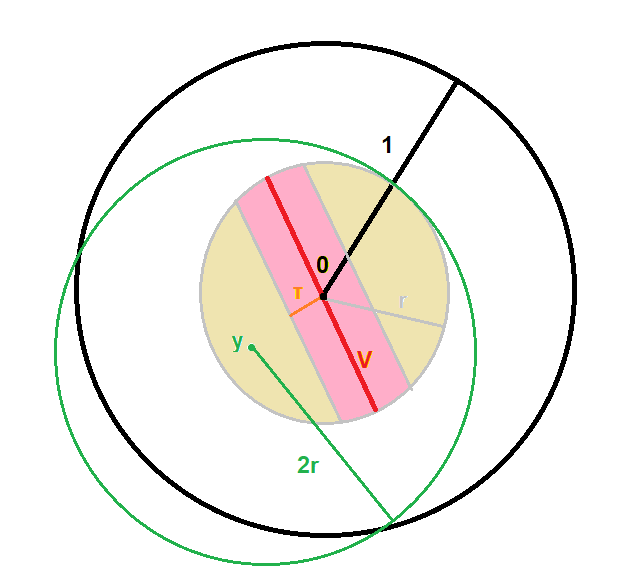
\includegraphics[scale = 0.6]{conesplit}
	\caption{The parameters $\tau \ll r \ll 1$ are chosen as a technical condition such that we have $B_{\tau} (V^k) \cap B_1 (0) \subseteq B_1 (0)$ and $B_r (0) \subseteq B_{2r} (y) \subseteq B_2 (0)$. Cone-splitting occurs in the ball $B_r (0)$.}
\end{center}	
\end{figure}


\begin{corollary}
	Let $f: B_2 (0) \to N^m$ be a stationary harmonic map with bounded energy $E[f] \leq \Lambda$. For every $\eta > 0$ and radii $\tau \ll r \ll 1$, there exists $\epsilon \ll_{n, N, \Lambda, \eta, \tau, r} 1$ such that if there exists $x \in B_r (0)$ such that 
	\begin{enumerate}
		\item $f$ is not $(\eta, r, k + 1)$-homogeneous at $x$, and
		\item $f$ is $(\epsilon, 2r, 0)$-homogeneous at $x$,\label{cor:coneb}
	\end{enumerate}
	then there exists a $k$-plane $V^k \subseteq \R^n$ such that 
		\[ \{ y \in B_r (0) : \text{$f$ is $(\epsilon, 2r, 0)$-homogeneous at $y$} \} \subseteq B_{\tau r} (V^k) .\] \label{cor:cone}
\end{corollary}

\begin{figure}[h]
\begin{center}
	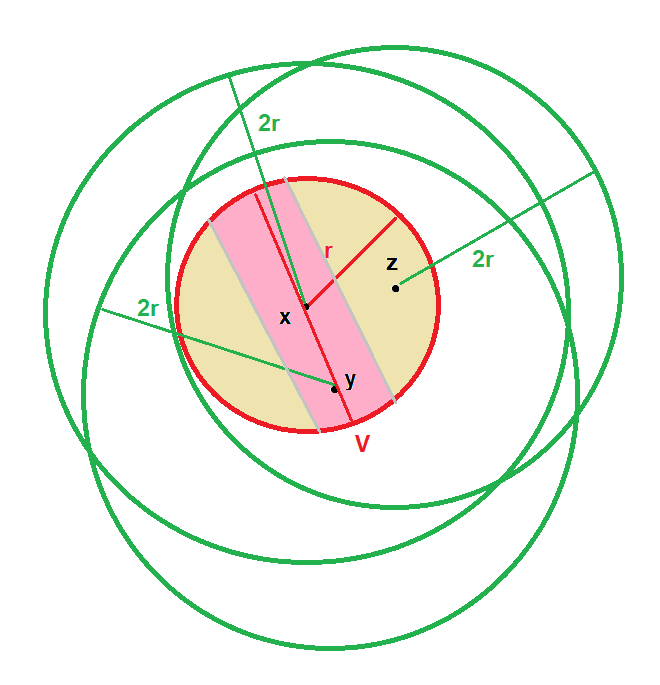
\includegraphics[scale = 0.6]{conesplit2}
	\caption{Sketch of proof for $k = 1$; assume otherwise, then there are $\{x_i\}_i, \{y_i\}_i, \{z_i\}_i$ satisfying (b) where $\{x_i, y_i, z_i\}$ are $\tau$-linearly independent, apply cone-splitting to get contradiction in the limit.}
\end{center}	
\end{figure}


\section{Stratification}
Our goal is to study the singular set of stationary and minimising harmonic maps. To this end, we stratify the singular set with regards to the homogeneity of the tangent map. Define
	\begin{align*}
		\operatorname{reg} f 
			&:= \{ x \in B_1 (0) : \text{$f$ is continuous in a neighborhood of $x$} \},\\
		 \operatorname{sing} f 
		 	&:= B_1 (0) \setminus \operatorname{reg} f.
	\end{align*}
The following is known about the singular set:
\begin{enumerate}
	\item $\cH^{n - 3} (\mathrm{sing} (f)) < \infty$ for minimising harmonic maps, \cite{SchoenUhlenbeck1982}. 
	\item $\cH^{n - 2} (\mathrm{sing} (f)) = 0$ for stationary harmonic maps, \cite{Bethuel1993,Lin1999}. 
	\item Let $B \subseteq \R^3$ be the unit ball, then for any non-constant $\phi : \partial B \to S^2$, there exists a weakly harmonic map in $W^{1, 2} (B, S^2)$ satisfying the Dirichlet problem for $\phi$ which is discontinuous everywhere, \cite{Riviere1995}.
\end{enumerate}


\subsection{Blow-up profile}

Let $f : \Omega \to N$ be a stationary harmonic map with bounded energy, define the blow-up at $y \in \Omega$ at scale $r > 0$ by
	\[ \mathsf T_{y, r} f (x) := f(y + r x). \]
We can extract a sub-sequence from the family $\{ \mathsf T_{y, r} f \}_{y, r}$ which converges weakly to a radially-invariant map, i.e. $0$-homogeneous. This shows that homogeneity is the correct infinitesimal structure to consider. Indeed, note that by a change of variables we can write
	\[ \theta_1 [\mathsf T_{y, r} f] (0) = \int_{B_1 (0)} |\nabla \mathsf T_{y, r} f|^2 \, \dV = \frac{1}{r^{n - 2}} \int_{B_r (y)} |\nabla f|^2 \, \dV = \theta_r [f](y). \]
It follows from the monotonicity of $\theta$ that the energy of the blow-ups is uniformly bounded in $r \ll 1$, hence there exists a sub-sequence converging weakly in $H^1 (B_1 (0) ; N)$ to $\mathsf T_y f : \R^n \to N$. Such a map is known as a \emph{tangent map}. Furthermore, we see from the monotonicity formula that for any $0 < R < 1$ we have
	\begin{align*}
		\int_R^1  \int_{\partial B_\rho (0)} \frac{1}{\rho^{n - 2}} \left| \frac{\partial \mathsf T_y f}{\partial \rho} \right|^2 d\rho \dA
			&=	 \theta_1 [\mathsf T_y f](0) - \theta_R [\mathsf T_y f] (0)\\
			&= \lim_{i \to \infty} \theta_1 [\mathsf T_{y, r_i} f] (0) - \theta_R [\mathsf T_{y, r_i} f] (0)= \lim_{i \to 0} \theta_{r_i} [f] (y) - \theta_{Rr_i} [ f](y) = 0. 
	\end{align*}	 
Since $R$ was arbitrary, we can conclude $\partial_\rho \mathsf T_y f\equiv 0$ on the entire ball $B_1 (0)$. Replacing the ball $B_1 (0)$ with $B_R (0)$ for any $R > 0$ and carrying through the same argument shows that convergence holds in $H^1_{\loc} (\R^n; N)$ and $\mathsf T_y f$ is in fact homogeneous of degree zero. 

\begin{remark}
	The uniqueness of tangent maps is an open problem. There are counter-examples due to \cite{White1991}.
\end{remark}

\begin{theorem}
	Let $f: B_2 (0) \to N$ be a stationary harmonic map with finite energy. Then $f$ is smooth in a neighborhood of $y \in B_2 (0)$ if and only if the tangent map is constant, i.e. $n$-homogeneous. 
\end{theorem}	

\begin{proof}
	This follows from $\epsilon$-regularity, c.f. \cite[Chapter 3.2]{Simon1996}. 
\end{proof}

	
\subsection{Main result}

Motivated by the results from the previous section, we have the following stratification of the singular set, 
	\[ \cS^k := \{ y \in B_2 (0) : \text{no tangent map at $y$ is $(k + 1)$-homogeneous}\}. \]
It is known that $\dim \cS^k \leq k$ and clear from construction that
	\[ \cS^0 \subseteq \cS^1 \subseteq \dots \subseteq \cS^{n - 1} = \operatorname{sing} f. \]
We refine the stratification, defining the \emph{quantitative $k$-th stratum} that is $\eta$-singular above scale $r > 0$ by 
	\[ \cS^k_{\eta, r} := \{ y \in B_2 (0) :  \text{$f$ is not $(\eta, s, k + 1)$-homogeneous at $y$ for all $r \leq s \leq 1$}  \}. \]	
It is clear from construction that
	\[ \cS^{k'}_{\eta, r} \subseteq \cS^k_{\eta', r'} , \qquad \cS^k = \bigcup_{\eta > 0} \bigcap_{r > 0} \cS^k_{\eta, r}\]
for $k' \leq k$, $\eta' \leq \eta$ and $r \leq r'$. Thus, to estimate the size of the singular set, it suffices to estimate the quantitative $k$-th stratums.
	
\begin{theorem}[Volume estimate on quantitative $k$-th stratum]
	Let $f: B_2 (0) \to N^m$ be a stationary harmonic map with bounded energy $E[f] \leq \Lambda$. Then for each $\eta > 0$,  
		\[ |B_r (\cS^k_{\eta, r})| \lesssim_{n, N, \Lambda, \eta} r^{n - k - \eta}. \]
		\label{thm:strat}
\end{theorem}

\section{Covering}
It suffices to prove the theorem for a discrete sequence of scales $r \in \{\gamma^j\}_j$ for some $\gamma \ll_{n, \eta} 1$ to be chosen later. This allows us to induct on scales to construct covers $\cC^k_{\eta, \gamma^j}$ of  $\cS^k_{\eta, \gamma^j}$ by balls of radius $\gamma^j$. At each stage of the induction, we decompose the stratum into disjoint subsets $E_{T^j} \subseteq B_1 (0)$ based on the behavior of points at various scales, and build up the cover $\cC^k_{\eta, \gamma^j}$ from sub-covers $\cC^k_{\eta, \gamma^j} (T^j) \subseteq \cC^k_{\eta, \gamma^j}$ of each subset, i.e.
	\begin{alignat*}{2}
		\cS^k_{\eta, \gamma^j} 
			&= \bigcup_{T^j \in \{0, 1\}^j} \cS^k_{\eta, \gamma^j} \cap E_{T^j},
			\\
		\cC^k_{\eta, \gamma^j}
			&= \bigcup	_{T^j \in \{0, 1\}^j} \cC^k_{\eta, \gamma^j} (T^j),	 \\
		 \cS^k_{\eta, \gamma^j} \cap E_{T^j} 
		 	&\subseteq \bigcup_{B_{\gamma^j} (x) \in \cC^k_{\eta, \gamma^j} (T^j)} B_{\gamma^j} (x).
	\end{alignat*}	
This covering will satisfy the following properties
	\begin{enumerate}
		\item by \textit{quantitative differentiation}, the number of non-empty $E_{T^j}$ and hence non-empty sub-covers $\cC^k_{\eta, \gamma^j} (T^j)$ is at most $j^Q$ for some $Q \lesssim_{n, \Lambda, \eta, \gamma, N} 1$, \label{prop:a}
		\item by \textit{quantitative cone-splitting}, each non-empty sub-cover $\cC^k_{\eta, \gamma^j} (T^j)$ consists of at most $(c_1 \gamma^{-n})^{Q} (c_0 \gamma^{-k})^{j - Q}$ balls of radius $\gamma^j$ for some dimensional constants $c_0, c_1 \lesssim_n 1$. \label{prop:b}
	\end{enumerate}
Note doubling the radii in the covering furnishes a covering of the tubular neighborhood $B_{\gamma^j} (\cS^k_{\eta, \gamma^j})$. We conclude the proof as follows, 
	\begin{align*}
		|B_{\gamma^j}(\cS^k_{\eta, \gamma^j})| 
			&\leq \sum_{\substack{T^j \in \{0, 1\}^j\\ E_{T_j} \neq \varnothing}} \sum_{B_{2\gamma^j} (x) \in \cC^k_{\eta, \gamma^j}} |B_{\gamma^j} (x)| \\
			&\lesssim_n j^Q (c_1 \gamma^{-n})^{Q} (c_0 \gamma^{-k})^{j - Q} (\gamma^j)^n \lesssim j^Q c_0^j (\gamma^j)^{n - k} \lesssim (\gamma^j)^{n - k - \eta},
	\end{align*}
where we choose our scale $\gamma$ to handle a dimensional constant, $\gamma \leq c_0^{-2/\eta}$, and can control a polynomial bound by an exponential bound, $j^Q \lesssim_{\gamma, \eta, Q} (\gamma^j)^{\eta/2}$. 

\subsection{Construction}

For each $x \in B_1 (0)$, we track the scales $\gamma^i$ at which the deviation is ``good'' and ``bad'' via the $j$-tuple $T^j (x)\in \{0, 1\}^j$, setting the $i$-th entry to be 
	\[
		T^j_i (x)
			:=
			\begin{cases}
				0, 		&\text{if $f$ is $(\epsilon, \gamma^i, 0)$-homogeneous at $x$} , \\
				1, 		&\text{if $f$ is not $(\epsilon, \gamma^i, 0)$-homogeneous at $x$},
			\end{cases}
	\]
where $\epsilon \ll 1$ will be chosen later to perform cone-splitting. For each $T^j \in \{0, 1\}^j$, define
	\[ E_{T^j} := \{ x \in B_1 (0) : T^j (x) = T^j \}. \]	
We construct the covers $\cC^k_{\eta, \gamma^j} (T^j)$ of $\cS^k_{\eta, \gamma^j} \cap E_{T^j}$ inductively in $j$. Denote $T^{j - 1}$ the $(j - 1)$-tuple obtained from $T^j$ by dropping the last entry. Then 
\begin{itemize}
	\item \textbf{Base:} Define 
		\[ \cC^k_{\eta, \gamma^0} := \cC^k_{\eta, \gamma^0} (T^0) := \{ B_1 (0)\}.\] 
		It is clear that $\cS^k_{\eta, \gamma^0} \cap E_{T^0}$ is covered by this collection of balls. 
	
	\item \textbf{Induction:} Suppose $\cC^k_{\eta, \gamma^{j - 1}} (T^{j - 1})$ is a cover of $\cS^k_{\eta, \gamma^{j - 1}} \cap E_{T^{j - 1}}$ by balls of radius $\gamma^{j - 1}$. For each ball $B_{\gamma^{j - 1}} (x) \in \cC^k_{\eta, \gamma^{j - 1}} (T^{j - 1})$, choose a minimal covering of $\cS^k_{\eta, \gamma^j} \cap E_{T^j} \cap B_{\gamma^{j - 1}} (x)$. 
	
	
	
	
\end{itemize}



\subsection{Quantitative differentiation}

\textit{A priori}, there could be as many as $2^j$-many non-empty $E_{T^j}$ in the decomposition. However, we can control the number of scales on which the scale-invariant energy defect is large by the pigeonhole principle, which by quantitative rigidity implies control over the number of ``bad'' scales, 
	\[ |T^j| \leq Q(n, N, \Lambda, \gamma, \epsilon) \qquad \text{whenever } E_{T^j} \neq \varnothing.\]
Since $\binom{j}{Q} \leq j^Q$, this would imply Property (\ref{prop:a}) of the covering. Let $\delta, r \ll_{n, N, \Lambda, \epsilon} 1$ be as in Lemma \ref{lem:rigid}, and fix $x \in E_{T^j}$. Recall the energy bound $E[f] \leq \Lambda$, so it follows from the monotonicity formula that
	\[ \sum_{[r\gamma^i, \gamma^i] \text{ disjoint}} \theta_{\gamma^i} (x) - \theta_{r\gamma^i} (x) \leq \Lambda. \]
The number of disjoint intervals of the form $[r \gamma^i, \gamma^i]$ is precisely $|\log_\gamma r|$, so by the pigeonhole principle and the bound above we have that
	\[  Q := |\log_\gamma r| \frac{\Lambda}{\delta}\]
bounds the number of scales such that
	\[ \theta_{\gamma^i} (x) - \theta_{r\gamma^i} (x) > \delta. \] 
By quantitative rigidity, these are the only ``bad'' scales in that if the inequality above does not hold, then $f$ must be $(\epsilon, \gamma^i, 0)$-homogeneous, so we conclude $|T^j| \leq Q$. 


\subsection{Cone-splitting}

Recall that the coverings $\cC^k_{\eta, \gamma^j} (T^j)$ are constructed inductively from minimal coverings of $\cS^k_{\eta, \gamma^j} \cap E_{T^j} \cap B_{\gamma^{j - 1}} (x)$ by balls of radius $\gamma^j$. There are two possible bounds for the number of balls in this covering:

\begin{enumerate}
	\item the efficient bound $c_0 \gamma^{-k}$. Recall from cone-splitting, namely Corollary \ref{cor:cone}, that if $\gamma^{j - 1}$ is a good scale, i.e. $T^j_{j - 1} = 0$ then there exists a $k$-plane $V^k \subseteq \R^n$ such that
		\[ \cS^k_{\eta, \gamma^j} \cap E_{T^j} \cap B_{\gamma^{j - 1}}(x) \subseteq B_{\frac{1}{1000} \gamma^j} (V^k) \cap  B_{\gamma^{j - 1}}(x). \]
		We can cover $V^k \cap B_{\gamma^{j - 1}} (x)$ by $c_0 \gamma^{-k}$ balls of radius $\gamma^j$ for some $c_0 \lesssim_n 1$, which in turn will cover a $\tfrac{1}{1000} \gamma^j$-neighborhood.
	
	\item the crude bound $c_1\gamma^{-n}$. Without knowing that a scale is good, we do not have control over the geometry of $\cS^k_{\eta, \gamma^j} \cap E_{T^j}$, so we naively cover $B_{\gamma^{j - 1}} (x)$ by $c_1 \gamma^{-n}$ balls of radius $\gamma^j$ for some $c_1 \lesssim_n 1$.
\end{enumerate}
By quantitative differentiation, we need only to use the crude bound for $Q$-many steps in the induction, while for the other steps we can apply the efficient bound. This proves Property (\ref{prop:b}) of the covering and thereby concludes the proof of Theorem \ref{thm:strat}.




\section{Regularity estimates}
The quantitative control over the singular stratum furnishes \textit{a priori} estimates for minimising harmonic maps. We first define the notion of regularity scale by 
	\[ r (x) := \sup \{ r > 0 : \sup_{B_r (x)} r |\nabla f| \leq 1  \}. \]
This allows us to partition the domain into ``good'' and ``bad'' sets depending on the behavior of $f$. Define
	\[ \cB_r := \{ x \in B_1 (0) : r(x) \leq r \}.  \]
The critical dimension for minimising harmonic maps is $n - 3$. Thus, given scale $r > 0$, if the map is sufficiently close to an $(n - 2)$-homogeneous, we expect the map to be essentially constant, and thus very smooth. More precisely 

\begin{lemma}[$\epsilon$-regularity]
	Let $f: B_2 (0) \to N$ be a minimising harmonic map with bounded energy $E[f] \leq \Lambda$. Then there exists $\eta \ll_{n, N, \Lambda, r} 1$ such that if $f$ is $(\eta, r, n - 2)$-homogeneous, then $r(0) \geq r$. In particular, 
		\[ \cB_r \subseteq \cS^{n - 3}_{\eta, r}. \]
\end{lemma}

\begin{theorem}
	Let $f : B_2 (0) \to N$ be a minimising harmonic map with bounded energy $E[f] \leq \Lambda$. Then we have the following 
		\[ |B_r (\cB_r)| \lesssim_{n, N, \lambda, \eta} r^{3 - \eta}. \]
	Moreover, for every $0 < p < 3$, we have
		\[ \int_{B_1 (0)} |\nabla f|^p \, \dV \leq \int_{B_1 (0)} r(x)^{-p} \, \dV \lesssim_{n, N, \Lambda, p} 1. \]	
\end{theorem}	

\begin{proof}
	Let $N \in 2^{\Z}$ denote a dyadic integer, then choosing $\eta \ll 3 - p$, we have
		\begin{align*}
			 \int_{B_1 (0)} r(x)^{-p} \, \dV
			 	&\leq \int_{r(x) \geq 1} r(x)^{-1} \, \dV + \sum_{N \leq 1} \int_{r(x) \sim N} r(x)^{-p} \, \dV \lesssim 1 + \sum_{N \leq 1} r^{3 - p - \eta} \lesssim 1. 
		\end{align*}
\end{proof}

\bibliographystyle{alpha}
\bibliography{external/biblio}
\end{document}